\documentclass[paper=a4,14pt]{scrartcl} % A4 paper and 11pt font size

\usepackage{multirow}

\usepackage{dsfont}

\usepackage{color}
\definecolor{darkgreen}{rgb}{0.0, 0.5, 0.0}

\usepackage[margin=0.425in]{geometry}
\usepackage{tikz}

\usepackage[nodisplayskipstretch]{setspace}
\setstretch{0.85}

\usepackage{amsmath}

\usepackage{wrapfig} % Allows in-line images 


\usepackage{hyperref}


\title{Ferroelectric phase field in Ferret (very short)}
\author{John Mangeri}

\begin{document}

\maketitle

\section*{Polarization evolution}
Starting from the second law of thermodynamics, the time-dependent Landau-Ginzburg equation can be derived for a ferroelectric body. It reads,
%
\begin{align}\label{TDLGD}
\frac{\partial \textbf{P}}{\partial t}&= - \Gamma_\textbf{P} \frac{\delta \mathcal{F}[\textbf{P}]}{\delta \textbf{P}} , \\ \nonumber
\end{align}
%
where $\mathcal{F}[\textbf{P}]$ is the system free energy \emph{functional} and $\textbf{P} =  \textbf{P}(\textbf{r},t)$ the polarization. The operator $\delta/\delta \textbf{P}$ denotes the variational (vector) derivative and the isotropic scalar $\Gamma_\textbf{P}$ defines the relaxation time globally. The total system free energy can be decomposed linearly into different contributions,
%
\begin{align}\label{freeE}
\mathcal{F}[\textbf{P}] &= F_\mathrm{bulk}[\textbf{P}] + F_\mathrm{gradient}[\textbf{P}] + F_\mathrm{elastic}[\mathbf{\varepsilon}] + F_\mathrm{electrostrictive}[\textbf{P},\mathbf{\varepsilon}] + F_\mathrm{elec}[\textbf{P}].\\ \nonumber
\end{align}
%
Each of these energy contributions carries different physics to the problem. The variable $\varepsilon$ is the elastic strain tensor with familiar relation
%
\begin{align}\label{strain}
\varepsilon_{ij} &= \frac{1}{2} \left[\frac{\partial u_i}{\partial x_j} +\frac{\partial u_j}{\partial x_i}\right].\\ \nonumber
\end{align}
%
where repeated indices are summed. The bulk energy,
%
\begin{align}\label{bulk}
&F_\mathrm{bulk} =  \alpha_1 \left(P_x^2 + P_y^2 + P_z^2 \right) + \alpha_{11} \left(P_x^4 + P_y^4 + P_z^4 \right) + \alpha_{12} \left(P_x^2 P_y^2 + P_y^2 P_z^2 + P_x^2 P_z^2 \right) \\ \nonumber
&+ \alpha_{111} \left(P_x^6 + P_y^6 + P_z^6 \right) + \alpha_{112} \left[P_x^4 \left(P_y^2 + P_z^2 \right) + P_y^4 \left(P_x^2 + P_z^2 \right) + P_z^4 \left(P_x^2 + P_y^2 \right) \right]  \\ \nonumber
&+ \alpha_{123} \left(P_x^2 P_y^2 P_z^2 \right),\\ \nonumber
\end{align}
%
defines the "double well" energy surface typical of centrosymmetric parent phase ferroelectrics. The gradient energy is
%
\begin{align}\label{grad}
&F_\mathrm{gradient}=\frac{1}{2} G_{11}  \left[ \left(\frac{\partial P_x}{\partial x} \right)^2 + \left(\frac{\partial P_y}{\partial y} \right)^2+\left(\frac{\partial P_z}{\partial z} \right)^2 \right] \\ \nonumber
&+  G_{12}  \left[\left(\frac{\partial P_x}{\partial x} \right)\left(\frac{\partial P_y}{\partial y} \right) + \left(\frac{\partial P_y}{\partial y} \right)\left(\frac{\partial P_z}{\partial z} \right) + \left(\frac{\partial P_x}{\partial x} \right)\left(\frac{\partial P_z}{\partial z} \right)\right] \\ \nonumber
&+ \frac{1}{2}G_{44} \left[\left(\left(\frac{\partial P_x}{\partial y} \right) + \left(\frac{\partial P_y}{\partial x} \right) \right)^2+ \left(\left(\frac{\partial P_y}{\partial z} \right) + \left(\frac{\partial P_z}{\partial y} \right) \right)^2+ \left(\left(\frac{\partial P_x}{\partial z} \right) + \left(\frac{\partial P_z}{\partial x} \right) \right)^2\right]\\ \nonumber
&+ \frac{1}{2} G_{44}' \left[\left(\left(\frac{\partial P_x}{\partial y} \right) - \left(\frac{\partial P_y}{\partial x} \right) \right)^2+\left(\left(\frac{\partial P_y}{\partial z} \right) - \left(\frac{\partial P_z}{\partial y} \right) \right)^2+\left(\left(\frac{\partial P_x}{\partial z} \right) - \left(\frac{\partial P_z}{\partial x} \right) \right)^2 \right]. \\ \nonumber
\end{align}
%
The elastic energy is the standard expression from linear elasticity\footnote{The elastic distortions due to the ferroelectric phase transition is considered a ''small strain'' problem as opposed to plastic deformations. Therefore, a reasonable approximation is to not allow the mesh itself to move. If one wants to allow the mesh grid to translate according to the elastic distortions from polarization evolution, the boolean flag \texttt{use$\_$displaced$\_$mesh} can be set true which will also increase the computational workload.},
%
\begin{align}\label{elastic}
F_\mathrm{elastic}&=\frac{1}{2} C_{ijkl} \varepsilon_{ij} \varepsilon_{kl}, \\ \nonumber
\end{align}
%
with couplings to polarization via
%
\begin{align}\label{elastic}
F_\mathrm{electrostrictive}&=\frac{1}{2} q_{ijkl} \varepsilon_{ij} P_k P_l. \\ \nonumber
\end{align}
%
The rank four tensors $C_{ijkl}$ and $q_{ijkl}$ reduce to their standard cubic symmetry form. Finally we consider the coupling of the polarization to an electrostatic potential that may arise from internal dipoles (the depolarization phenomena) or an applied field,
%
\begin{align}\label{elastic}
F_\mathrm{elec}&= -\frac{1}{2} P_k \frac{\partial \Phi}{\partial x_k}. \\ \nonumber
\end{align}
%
All expressions coded in Ferret are consistent with Ref. \cite{Li2001} and \cite{Hlinka2006} for lead titanate and barium titante respectively. 
%
They have been tested in bulk (3D periodic) and in a film (3D calculation with 2D periodicity).
%
For example, consider $\mathrm{BaTiO}_3$ potential \cite{Hlinka2006} for a single domain at T = 298 K, the spontaneous polarization is published as $P_s = 0.265$ $\mathrm{C}/\mathrm{m}^2$ and the Ferret result is $P_s = 0.2653$ $\mathrm{C}/\mathrm{m}^2$. Published (and Ferret) spontaneous strains are $\varepsilon_{||} = 7.77\times10^{-3}(7.38\times10^{-3})$ and $\varepsilon_{||} = -3.18\times10^{-3}(-3.165\times10^{-3})$ showing good agreement.
%
%The free energy functional coefficients should be chosen as "stress-free" and not the Legendre transformed "strain-free" formulation.

\section*{Coupled problem}

In order to ensure both mechanical and electrostatic equilibrium, the following equations are also evolved concurrently with Eq. \ref{TDLGD},
\begin{align}\label{aux}
\frac{\partial u_i}{\partial t}&= \frac{\partial \sigma_{ij}^\mathrm{total}}{\partial x_j}. \\ \nonumber
\frac{\partial \Phi}{\partial t}&= \epsilon_b\frac{\partial^2 \Phi}{\partial x_i \partial x_i}-\frac{\partial P_j}{\partial x_j}, \\ \nonumber
\end{align}
%
where the stress has two components, one from the elastic contribution and another due to electrostriction. In the quasi-static limit, $\partial u_i / \partial t = 0$ and $\partial \Phi / \partial t = 0$ and these equations reduce to the familiar stress-divergence\footnote{Note that the stress-divergence equation is of the form,

$$\frac{\partial \sigma_{ij}^\mathrm{total}(\textbf{r})}{\partial x_j}  = C_{ijkl}\left[\varepsilon_{kl}(\textbf{r}) - Q_{klmn}P_m(\textbf{r}) P_n(\textbf{r})\right] = 0$$} and Poisson equations with $\epsilon_b$ being the background permitivitty contribution from core electrons \cite{Hlinka2006}. 
%
Solving them at every time step allows for elastic strain and electric field to follow the polarization evolution and penalizes any evolution that would increase the total free energy (for example, charge domain wall formation).
%
Allowing time-dependence on the secondary variables can sometimes speed up convergence somewhat, so it is left as an option for the user.

\section*{Simulations}
%
%
\begin{wrapfigure}{r}{0.5\textwidth}
  \begin{center}
\vspace{-50pt}
    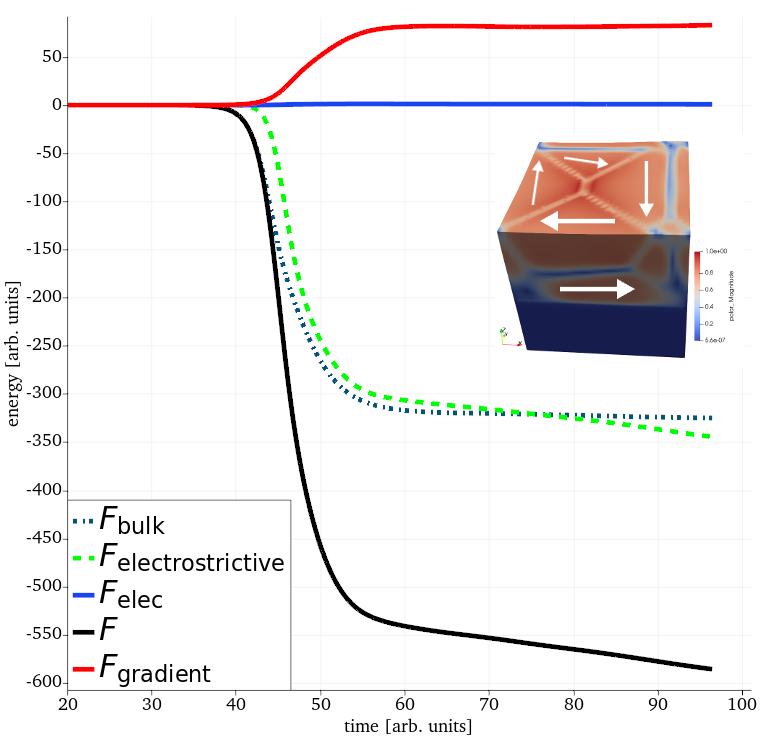
\includegraphics[width=0.42\textwidth]{time_evol.png}
  \end{center}
  \caption{Example of time evolution of the free energy contributions given a random paraelectric IC. The gradient energy grows resulting in the domain pattern of the inset.}
\end{wrapfigure}
%
When evolving Eq. \ref{TDLGD} to an energy minima, all of the above equations are cast into weak form residual contributions sufficient for finite element analysis and Newton or almost-Newton steppers are used to solve at every time step.
%
The initial condition (IC) and boundary conditions on $\textbf{P}(\textbf{r},t), \textbf{u},$ and $\Phi$ must be defined to gaurantee diffusive gradient flow from high ($t=t_0$) to low energy.
%
A common initial condition on $\textbf{P}$ is to set a random condition such that $|\textbf{P}(\textbf{r},t=t_0)| \ll 0 $. This is essentially the ''paraelectric'' high symmetry structure above the Curie temperature.
%
Then, energy is kicked out at every time step according to Eq. \ref{TDLGD}
%


%
MOOSE has full functionality to define spatially dependent initial conditions. As such, another common initial condition for the polar field is to assume a sine wave profile and the solution of Eq. \ref{TDLGD} will lock in the polarization into a domain pattern assuming full periodic boundary conditions.
%
The boundary conditions can be Dirichlet, integrated, Neumann, periodic, or mixed. Function (spatiotemporal) definitions of all of these are allowed and it is quite trivial to write your own.
%
Time integration schemes for Eq. \ref{TDLGD} are numerous and the user has access to many (implicit and explicit Euler, backwards finite differencing, Crank-Nicolson, etc all with the possible for adaptive stepping).
%
Adaptive mesh refinement is also possible but it is currently not tested very extensively for Ferret calculations.
%
Hysteresis loops can be performed in quasi-static or fully dynamical modes (with time dependent boundary conditions) with or without thermal noise to help activate switching over the local energy barriers.

%
\subsection*{Periodic boundary conditions}
%
As stated above, periodic boundary conditions are allowed within MOOSE/Ferret. But since we explicitly solve for the displacement vector $\textbf{u}$ additional care must be taken to ensure the strain field is periodic.
%
Following Biswas \emph{et al} \cite{Biswas2020}, the strain-periodic formulation in MOOSE/Ferret introduces a volumetric deformation instead of imposing additional constraints at the boundary. 
%
A similar approach exists in Ref. \cite{Muench2019}. This reference is worth a read to understand the delicate nature of implementing periodic boundary conditions in ferroelectric structure without the use the FFT-based codes which automatically assume periodicity in the strain field due to the assumption of a regular computational volume.
%
It is advantageous computationally as only six extra degrees of freedom are needed instead of a multiplier per variable per boundary node.
%

%
While still maintaining the periodicity, volume and shape distortion are allowed which relax the elastic stresses along the periodic direction. 
%
Note that when someone says "stress free" within a ferroelectric unit cell, they mean the stress arising from the polar coupling internally within the crystal zeros the stress due to the elastic disortion which accomodates the polar field (volumetric tetragonal distortion of the unit cell for example).
%
However, at the domain walls or free surfaces some stress may accumulate which corresponds to a minimized free energy. 
%
Therefore, the care must be taken to allow for stress minimization inside domain structure but also allowing the computational cell to deform its shape and volume to minimize the total system energy.
%
Within MOOSE/Ferret, the following integral equation,
%
\begin{align}\label{ode}
\int\limits_V d^3\textbf{r} \left[\sigma_{k}^\mathrm{total}(\textbf{P},\varepsilon) - \sigma_{k}^\mathrm{appl} \right] = 0, \\ \nonumber
\end{align}
%
where k = 1, 2, 3, 4, 5, 6 = xx, yy, zz, xy, xz, yz is solved. 
%
\begin{figure}[h]\centering
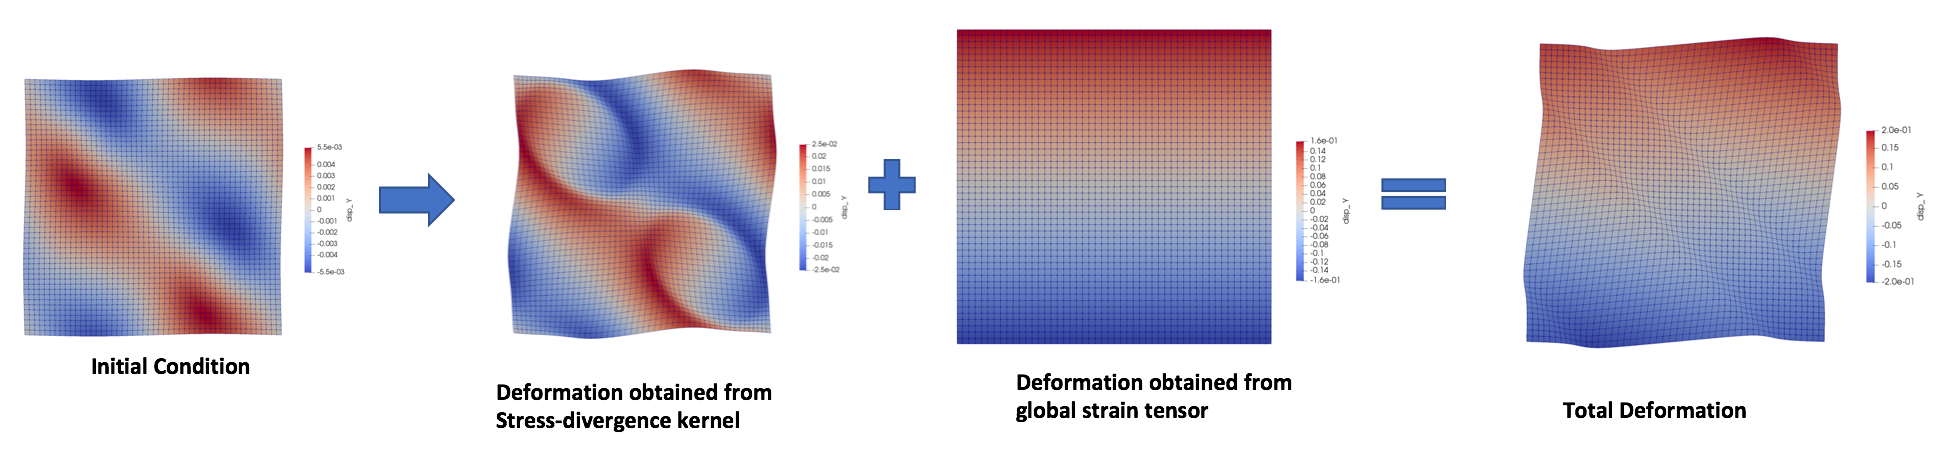
\includegraphics[width=19cm]{example_horizontal.png}\caption{Example of global strain system in action. The final image shows the conformation including both a local and global contribution. The curvature of the periodic boundaries clearly indicating the correct traction condition ($\textbf{t} = \textbf{n}\cdot \sigma$).}\label{fig2}
\end{figure}
%
The total stress tensor component $\sigma_{k}^\mathrm{total}$ is comprised of both an electrostrictive and elastic part. When $\sigma_{k}^\mathrm{total}$ is zero \emph{locally}, the crystal can be considered stress free \emph{locally}.
%
The \texttt{GlobalStrain} system introduces six new components of a global strain tensor with the familiar definition,
%
\begin{align}
\varepsilon_{ij}^g(\textbf{r}) = \frac{1}{2}\left(\frac{\partial u_i^g(\textbf{r})}{\partial x_j}+\frac{\partial u_j^g(\textbf{r})}{\partial x_i}\right),
\end{align}
%
to zero Eq. \ref{ode} by solving a scalar ODE in between time-steps.
%
Each of the six components of the strain tensor are degrees of freedom for the approach to enforce strain periodicity. The values of the auxilliary variables $\textbf{u}^g$ computed using the definition,
%
\begin{align}
\textbf{u}^g(\textbf{r}) = (\textbf{r} - \textbf{r}_0)\cdot\varepsilon^g.
\end{align}
%
where is $\textbf{r}_0$ is an arbitrary reference node that does not influence the calculation. An pictographical example of this is provided in Fig. \ref{fig2}.





%\section*{Example: single domain BTO (T=298K)}
%
%In the case of monodomain (fully 3D PBC) tetragonal room temp BTO (functional from Hlinka \emph{et al} \cite{Hlinka2006}) we find $P_0 = 0.265229$(published result is 0.2650), zero components otherwise. 
%%
%The elastic stress tensor gives $\sigma_{xx} = \sigma_{yy} = -0.052$ GPa. Shearing stress are all zero. The stress along P is $\sigma_{zz} = +0.99$ GPa. Similarly, shearing strains are all zero. Longitudinal strain is el=7.738e-3 (published result is el=7.77e-3) and transverse strain is ep=-3.165e-3 where the published result is ep = -3.18e-3. Calculation of the expected eigenstress,
%%
%$$\sigma_{ij}^0 = C_{ijkl} Q_{klmn} P_m P_n, $$
%%
%gives equal and opposite values thus the structure is stress-free ($\sigma_\mathrm{ij}^\mathrm{total} = \sigma_{ij} - \sigma_{ij}^0 = 0$) as expected for a RVE of monodomain BTO.
%%


%\section{AMR:}
%
%AMR with Nemesis mesh is particularly challenging to deal with the data flow. A 256 processor job stepping 210 times saving every 10 steps with aggressive AMR generates 256*21+1 = 5377 files (all around 10-40 kb each). Luckily, they are grouped in a smart way and one only needs to load any of the processor files but only the last AMR step. The calculation is pretty efficient ($10^3$ sec for a 40x40x10 nm block with 1nm mesh resolution).


\begin{thebibliography}{1}
%
\bibitem{Li2001}
Y.~L.~Li, S.~Y.~Hu, Z.~K.~Liu, and L.-Q.~Chen,
\newblock \emph{Appl.~Phys.~Lett.} \textbf{78} 492--500 (2001).
%
\bibitem{Hlinka2006}
J.~Hlinka, and P.~Marton,
\newblock \emph{Phys.~Rev.~B} \textbf{74} 104104 (2006).
%
\bibitem{Biswas2020}
S.~Biswas, D.~Schwen, and J.~Hales,
\newblock \emph{Fin. Elem. Anal. Design} \textbf{179} 103436 (2020).
%
\bibitem{Muench2019}
I.~Muench, A.~Renuka Balakrishna, and J.~E.~Huber,
\newblock \emph{Arch. Appl. Mech.} \textbf{89} 955–972 (2019).
%




\end{thebibliography}
\end{document}
